\section{XUPV2}

En este proyecto se usa la tarjeta Xilinx University Program Virtex 2 (XUPV2).
La tarjeta de desarrollo \emph{XUPV2} es un dispositivo con características
para la evaluación de proyectos de  propósito general, la plataforma de
desarrollo cuenta con memoria incrustrada e interfaces estándar de la industria
de conectividad. Cuenta con el dispositivo FPGA \emph{Virtex-2}.

\subsection{Características de la  tarjeta de desarrollo \emph{XUPV2} }

Las características con las que cuenta la tarjeta de desarrollo son:

\begin{itemize}
\item FPGA Virtex-2 Pro XC2VP30  con 30,816 celdas lógicas, 136 18-bit multiplicadores,
 2,448Kb bloques de RAM y 2 Procesadores PowerPC.
\item DDR SDRAM DIMM de hasta  2Gbytes de RAM
\item Puerto Ethernet 10/100
\item Puerto USB2 
\item Lector de tarjetas Compact Flash
\item Puerto de video XSGA
\item Audio Codec
\item Puertos SATA, S/2 y RS-232
\end{itemize}


\begin{figure}[h!]
 \centering
 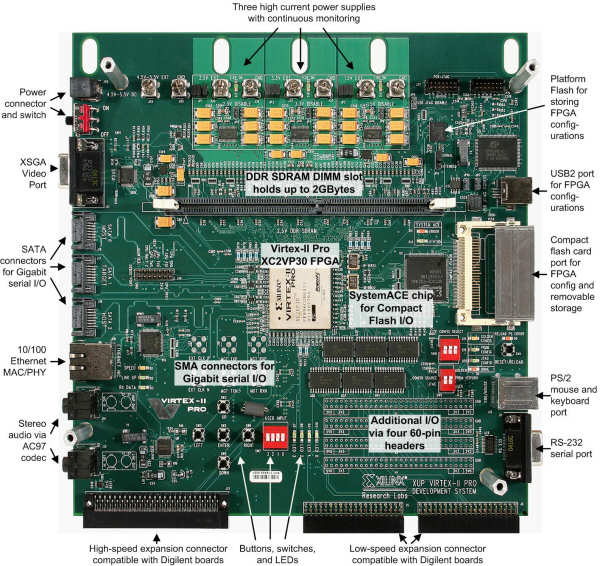
\includegraphics{./figuras/V2.jpg}
 % V5.jpg: 1000x805 pixel, 72dpi, 35.28x28.40 cm, bb=0 0 1000 805
  \caption{Tarjeta de desarrollo Virtex-II Pro Development System}
 \label{XUPV502}
\end{figure}


La lista detallada de características de la tarjeta de desarrollo \emph{XUPV2}
puede ser consultada en la dirección : 
\begin{center}
 \url{http://www.xilinx.com/univ/xupv2p.html}
\end{center}
